%%%%%%%%%%%%%%%%%%%%%%%%%%%%%%%%%%%%%%%%%%%%%%%%%%%%%%%%%%%%%%%
% National Road Safety Hackathon 2025 - Project Presentation
% Project: Road Safety Intervention GPT
% Team: The Silicon Savants
% Members: Gyan Chandra (IIITDM Kancheepuram) & Dristi Singh (KIIT University)
% GitHub: https://github.com/gyanchandra2910/RoadSafety
%%%%%%%%%%%%%%%%%%%%%%%%%%%%%%%%%%%%%%%%%%%%%%%%%%%%%%%%%%%%%%%

\documentclass[aspectratio=169,12pt]{beamer}

% Theme and Color Settings - AI/Tech Blue-Gray Style
\usetheme{Madrid}
\usecolortheme{default}

% Custom AI-Theme Colors
\definecolor{aiblue}{RGB}{33,150,243}
\definecolor{darkblue}{RGB}{13,71,161}
\definecolor{techgray}{RGB}{96,125,139}
\definecolor{lightgray}{RGB}{236,239,241}
\definecolor{accentcyan}{RGB}{0,188,212}

\setbeamercolor{palette primary}{bg=darkblue,fg=white}
\setbeamercolor{palette secondary}{bg=aiblue,fg=white}
\setbeamercolor{palette tertiary}{bg=techgray,fg=white}
\setbeamercolor{structure}{fg=darkblue}
\setbeamercolor{frametitle}{bg=darkblue,fg=white}
\setbeamercolor{title}{bg=darkblue,fg=white}
\setbeamercolor{block title}{bg=aiblue,fg=white}
\setbeamercolor{block body}{bg=lightgray,fg=black}

% Packages
\usepackage[utf8]{inputenc}
\usepackage{graphicx}
\usepackage{tikz}
\usepackage{listings}
\usepackage{booktabs}
\usepackage{hyperref}
\usepackage{fontawesome5}

\usetikzlibrary{shapes.geometric, arrows, positioning, shadows}

% Footer with hackathon info
\setbeamertemplate{footline}{
  \leavevmode%
  \hbox{%
  \begin{beamercolorbox}[wd=.5\paperwidth,ht=2.5ex,dp=1ex,left]{author in head/foot}%
    \hspace*{2ex}\footnotesize National Road Safety Hackathon 2025 | IIT Madras - CoERS
  \end{beamercolorbox}%
  \begin{beamercolorbox}[wd=.5\paperwidth,ht=2.5ex,dp=1ex,right]{date in head/foot}%
    \footnotesize The Silicon Savants\hspace*{2ex}
  \end{beamercolorbox}}%
  \vskip0pt%
}

% Title Information
\title[\textbf{Road Safety Intervention GPT}]{Road Safety Intervention GPT}
\subtitle{AI-Powered Identification of Road Safety Interventions}
\author[Gyan Chandra \& Dristi Singh]{
    \textbf{Gyan Chandra} \\ \small IIITDM Kancheepuram \\[0.2cm]
    \textbf{Dristi Singh} \\ \small KIIT University \\[0.3cm]
    \textit{Team: The Silicon Savants}
}
\institute[IIT Madras]{
    \textbf{National Road Safety Hackathon 2025}\\
    Centre of Excellence for Road Safety (CoERS)\\
    IIT Madras
}
\date{November 2025}

%%%%%%%%%%%%%%%%%%%%%%%%%%%%%%%%%%%%%%%%%%%%%%%%%%%%%%%%%%%%%%%
% Begin Document
%%%%%%%%%%%%%%%%%%%%%%%%%%%%%%%%%%%%%%%%%%%%%%%%%%%%%%%%%%%%%%%

\begin{document}

%%%%%%%%%%%%%%%%%%%%%%%%%%%%%%%%%%%%%%%%%%%%%%%%%%%%%%%%%%%%%%%
% SLIDE 1: WELCOME
%%%%%%%%%%%%%%%%%%%%%%%%%%%%%%%%%%%%%%%%%%%%%%%%%%%%%%%%%%%%%%%

\begin{frame}[plain]
\titlepage
\vspace{-0.8cm}
\begin{center}
    \textcolor{aiblue}{\rule{10cm}{2pt}}
    
    \vspace{0.3cm}
    {\large \textbf{Problem Statement 1.3}}\\
    \vspace{0.1cm}
    \textit{Identification of Road Safety Interventions using GPT-based AI Tool}
    
    \vspace{0.4cm}
    
    % Logo placeholders
    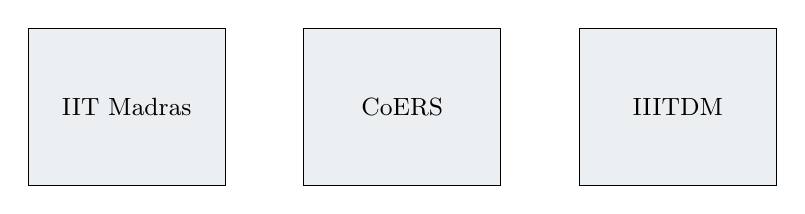
\begin{tikzpicture}
        \node[draw, rectangle, fill=lightgray, minimum width=2.5cm, minimum height=2cm] at (0,0) {\small IIT Madras};
        \node[draw, rectangle, fill=lightgray, minimum width=2.5cm, minimum height=2cm] at (3.5,0) {\small CoERS};
        \node[draw, rectangle, fill=lightgray, minimum width=2.5cm, minimum height=2cm] at (7,0) {\small IIITDM};
    \end{tikzpicture}
    
    \vspace{0.3cm}
    
    {\footnotesize \faGithub~\textcolor{aiblue}{\href{https://github.com/gyanchandra2910/RoadSafety}{github.com/gyanchandra2910/RoadSafety}}}
\end{center}
\end{frame}

%%%%%%%%%%%%%%%%%%%%%%%%%%%%%%%%%%%%%%%%%%%%%%%%%%%%%%%%%%%%%%%
% SLIDE 2: PROBLEM STATEMENT & MOTIVATION
%%%%%%%%%%%%%%%%%%%%%%%%%%%%%%%%%%%%%%%%%%%%%%%%%%%%%%%%%%%%%%%

\begin{frame}{Problem Statement \& Motivation}
\framesubtitle{Why AI-Driven Road Safety Intervention Automation?}

\begin{columns}[T]
\begin{column}{0.48\textwidth}
    \begin{block}{The Crisis}
        \begin{itemize}
            \item \textbf{150,000+} annual road fatalities in India
            \item \textbf{11\%} of global road deaths
            \item \textbf{5 lakh+} people injured yearly
            \item Economic loss: \textbf{3-5\% of GDP}
        \end{itemize}
    \end{block}
    
    \vspace{0.3cm}
    
    \begin{block}{Current Challenges}
        \begin{itemize}
            \item \textcolor{aiblue}{\faExclamationTriangle}~Manual identification of interventions
            \item \textcolor{aiblue}{\faClock}~Time-consuming expert analysis
            \item \textcolor{aiblue}{\faQuestion}~Inconsistent recommendations
            \item \textcolor{aiblue}{\faDatabase}~Limited access to IRC standards
        \end{itemize}
    \end{block}
\end{column}

\begin{column}{0.48\textwidth}
    \begin{alertblock}{Why Automation?}
        \textbf{Need for intelligent, data-driven decision support system}
        \begin{itemize}
            \item Fast identification of safety measures
            \item IRC-compliant recommendations
            \item Context-aware AI reasoning
            \item Accessible to all stakeholders
        \end{itemize}
    \end{alertblock}
    
    \vspace{0.3cm}
    
    \begin{block}{Target Users}
        \begin{itemize}
            \item \faRoad~Highway Engineers
            \item \faUsers~Traffic Authorities
            \item \faChartLine~Policy Makers
            \item \faUniversity~Researchers
        \end{itemize}
    \end{block}
\end{column}
\end{columns}

\vspace{0.3cm}
\begin{center}
    \textcolor{darkblue}{\textit{\textbf{"Faster interventions = Lives saved"}}}
\end{center}

\end{frame}

%%%%%%%%%%%%%%%%%%%%%%%%%%%%%%%%%%%%%%%%%%%%%%%%%%%%%%%%%%%%%%%
% SLIDE 3: OBJECTIVE
%%%%%%%%%%%%%%%%%%%%%%%%%%%%%%%%%%%%%%%%%%%%%%%%%%%%%%%%%%%%%%%

\begin{frame}{Objective}
\framesubtitle{Intelligent Intervention Recommendation System}

\begin{center}
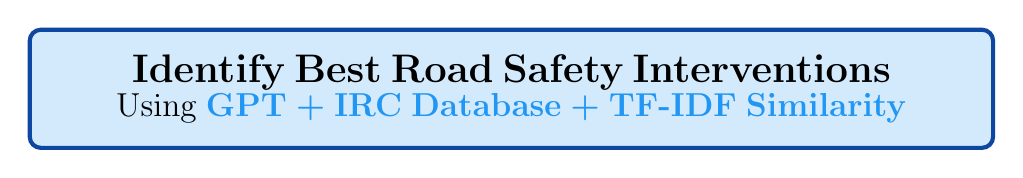
\begin{tikzpicture}[node distance=0.5cm]
    % Main objective box
    \node[rectangle, draw=darkblue, fill=aiblue!20, text width=12cm, text centered, rounded corners, line width=1.5pt, minimum height=1.5cm] (main) {
        \Large \textbf{Identify Best Road Safety Interventions}\\
        \large Using \textcolor{aiblue}{\textbf{GPT + IRC Database + TF-IDF Similarity}}
    };
\end{tikzpicture}
\end{center}

\vspace{0.5cm}

\begin{columns}[T]
\begin{column}{0.48\textwidth}
    \begin{block}{Primary Goals}
        \begin{enumerate}
            \item \textbf{Automate} intervention identification
            \item \textbf{Provide} IRC-compliant solutions
            \item \textbf{Generate} AI-backed explanations
            \item \textbf{Reduce} response time to \textcolor{aiblue}{<2 seconds}
        \end{enumerate}
    \end{block}
    
    \vspace{0.3cm}
    
    \begin{block}{Input \faArrowRight~Output}
        \textbf{Input:}\\
        Natural language description of road safety issue
        
        \vspace{0.2cm}
        
        \textbf{Output:}\\
        Ranked interventions + GPT explanations + IRC references
    \end{block}
\end{column}

\begin{column}{0.48\textwidth}
    \begin{block}{Key Features}
        \begin{itemize}
            \item \textcolor{aiblue}{\faBrain}~\textbf{AI-Powered}: GPT-3.5 reasoning
            \item \textcolor{aiblue}{\faSearch}~\textbf{Smart Search}: TF-IDF similarity
            \item \textcolor{aiblue}{\faBook}~\textbf{IRC Standards}: Compliant solutions
            \item \textcolor{aiblue}{\faChartBar}~\textbf{Scored Results}: Relevance ranking
            \item \textcolor{aiblue}{\faTachometerAlt}~\textbf{Fast}: Sub-2-second response
            \item \textcolor{aiblue}{\faDesktop}~\textbf{Web-Based}: Accessible anywhere
        \end{itemize}
    \end{block}
    
    \vspace{0.3cm}
    
    \begin{alertblock}{Innovation}
        \textbf{Hybrid AI Approach:}\\
        Traditional ML + Modern LLM
    \end{alertblock}
\end{column}
\end{columns}

\end{frame}

%%%%%%%%%%%%%%%%%%%%%%%%%%%%%%%%%%%%%%%%%%%%%%%%%%%%%%%%%%%%%%%
% SLIDE 4: PROPOSED SOLUTION / SYSTEM ARCHITECTURE
%%%%%%%%%%%%%%%%%%%%%%%%%%%%%%%%%%%%%%%%%%%%%%%%%%%%%%%%%%%%%%%

\begin{frame}{Proposed Solution: System Architecture}
\framesubtitle{AI-Powered Hybrid Recommendation Engine}

\begin{center}
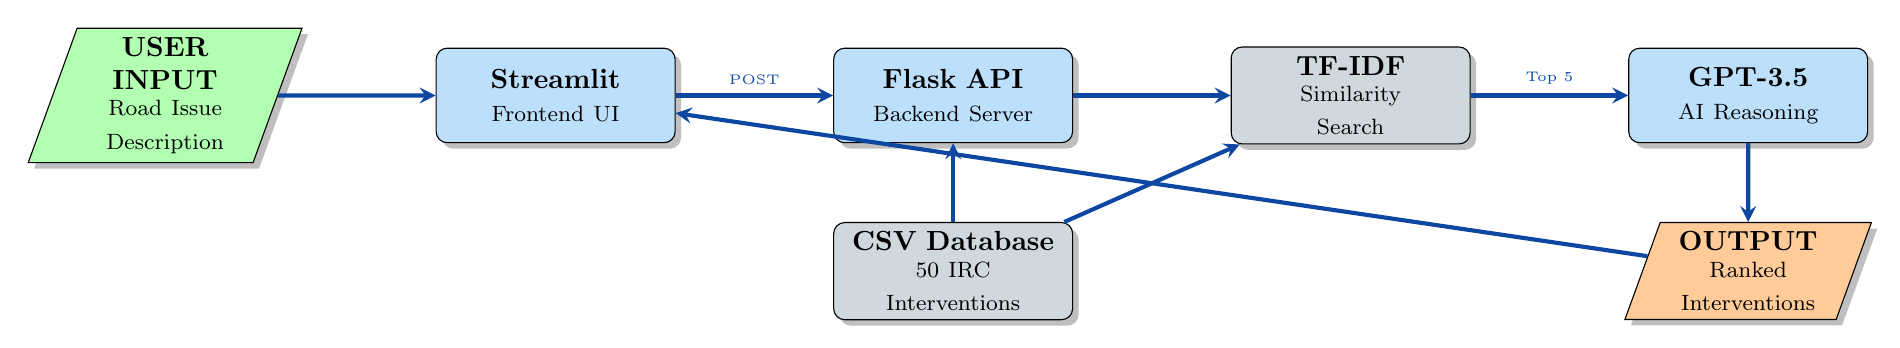
\begin{tikzpicture}[
    node distance=1.8cm and 2cm,
    block/.style={rectangle, draw, fill=aiblue!30, text width=2.8cm, text centered, rounded corners, minimum height=1.2cm, drop shadow},
    process/.style={rectangle, draw, fill=techgray!30, text width=2.8cm, text centered, rounded corners, minimum height=1.2cm, drop shadow},
    io/.style={trapezium, trapezium left angle=70, trapezium right angle=110, draw, fill=green!30, text width=2cm, text centered, minimum height=1cm, drop shadow},
    output/.style={trapezium, trapezium left angle=70, trapezium right angle=110, draw, fill=orange!40, text width=2cm, text centered, minimum height=1cm, drop shadow},
    arrow/.style={->, >=stealth, line width=1.5pt, color=darkblue}
]
    % Input
    \node[io] (input) {\textbf{USER INPUT}\\{\footnotesize Road Issue\\Description}};
    
    % Streamlit UI
    \node[block, right=of input] (ui) {\textbf{Streamlit}\\{\footnotesize Frontend UI}};
    
    % Flask API
    \node[block, right=of ui] (api) {\textbf{Flask API}\\{\footnotesize Backend Server}};
    
    % Database
    \node[process, below=1cm of api] (db) {\textbf{CSV Database}\\{\footnotesize 50 IRC\\Interventions}};
    
    % TF-IDF Search
    \node[process, right=of api] (tfidf) {\textbf{TF-IDF}\\{\footnotesize Similarity\\Search}};
    
    % GPT Processing
    \node[block, right=of tfidf] (gpt) {\textbf{GPT-3.5}\\{\footnotesize AI Reasoning}};
    
    % Output
    \node[output, below=1cm of gpt] (output) {\textbf{OUTPUT}\\{\footnotesize Ranked\\Interventions}};
    
    % Arrows
    \draw[arrow] (input) -- (ui);
    \draw[arrow] (ui) -- node[above, font=\tiny] {POST} (api);
    \draw[arrow] (api) -- (tfidf);
    \draw[arrow] (db) -- (api);
    \draw[arrow] (db) -- (tfidf);
    \draw[arrow] (tfidf) -- node[above, font=\tiny] {Top 5} (gpt);
    \draw[arrow] (gpt) -- (output);
    \draw[arrow] (output) -- (ui);
    
\end{tikzpicture}
\end{center}

\vspace{0.4cm}

\begin{block}{Workflow Steps}
    \begin{enumerate}
        \item User describes road safety issue via \textcolor{aiblue}{\textbf{Streamlit UI}}
        \item Query sent to \textcolor{aiblue}{\textbf{Flask backend API}}
        \item \textcolor{aiblue}{\textbf{TF-IDF}} searches 50 IRC interventions in CSV database
        \item Top 5 matches sent to \textcolor{aiblue}{\textbf{GPT-3.5}} with context (problem + IRC clauses)
        \item GPT generates \textcolor{aiblue}{\textbf{professional explanation}} referencing standards
        \item System returns \textcolor{aiblue}{\textbf{ranked results + AI insight}} to user
    \end{enumerate}
\end{block}

\end{frame}

%%%%%%%%%%%%%%%%%%%%%%%%%%%%%%%%%%%%%%%%%%%%%%%%%%%%%%%%%%%%%%%
% SLIDE 5: IMPLEMENTATION
%%%%%%%%%%%%%%%%%%%%%%%%%%%%%%%%%%%%%%%%%%%%%%%%%%%%%%%%%%%%%%%

\begin{frame}{Implementation}
\framesubtitle{Technology Stack \& Development}

\begin{columns}[T]
\begin{column}{0.48\textwidth}
    \begin{block}{Tech Stack}
        \begin{table}
        \footnotesize
        \begin{tabular}{ll}
            \toprule
            \textbf{Component} & \textbf{Technology} \\
            \midrule
            \faCode~Language & Python 3.13 \\
            \faServer~Backend & Flask 3.0+ \\
            \faDesktop~Frontend & Streamlit 1.28+ \\
            \faBrain~AI Engine & OpenAI GPT-3.5 \\
            \faSearch~Search & TF-IDF (scikit-learn) \\
            \faDatabase~Data & Pandas, NumPy \\
            \faFile~Database & CSV (50 records) \\
            \faCodeBranch~Version Control & Git/GitHub \\
            \bottomrule
        \end{tabular}
        \end{table}
    \end{block}
    
    \vspace{0.3cm}
    
    \begin{block}{Key Libraries}
        \begin{itemize}
            \item \texttt{openai} - GPT API integration
            \item \texttt{flask-cors} - Cross-origin support
            \item \texttt{scikit-learn} - TF-IDF vectorization
            \item \texttt{python-dotenv} - Config management
        \end{itemize}
    \end{block}
\end{column}

\begin{column}{0.48\textwidth}
    \begin{block}{Backend (Flask API)}
        \begin{itemize}
            \item \texttt{POST /recommend}\\
            {\footnotesize Main recommendation endpoint}
            \item \texttt{GET /health}\\
            {\footnotesize Server status monitoring}
            \item OpenAI GPT-3.5-turbo integration
            \item TF-IDF similarity matching
            \item IRC-compliant response format
        \end{itemize}
    \end{block}
    
    \vspace{0.3cm}
    
    \begin{block}{Frontend (Streamlit UI)}
        \begin{itemize}
            \item Natural language input form
            \item Real-time API communication
            \item Color-coded relevance indicators
            \item Expandable result cards
            \item AI explanation display
        \end{itemize}
    \end{block}
    
    \vspace{0.3cm}
    
    \begin{block}{Dataset}
        \textbf{GPT\_Input\_DB.csv}\\
        50 curated interventions with IRC clauses
    \end{block}
\end{column}
\end{columns}

\vspace{0.3cm}

\begin{center}
    \textcolor{darkblue}{\faGithub~\textbf{GitHub Repository:}} \textcolor{aiblue}{\href{https://github.com/gyanchandra2910/RoadSafety}{github.com/gyanchandra2910/RoadSafety}}
\end{center}

\end{frame}

%%%%%%%%%%%%%%%%%%%%%%%%%%%%%%%%%%%%%%%%%%%%%%%%%%%%%%%%%%%%%%%
% SLIDE 6: RESULTS & OUTPUTS
%%%%%%%%%%%%%%%%%%%%%%%%%%%%%%%%%%%%%%%%%%%%%%%%%%%%%%%%%%%%%%%

\begin{frame}{Results \& Outputs}
\framesubtitle{System Interface \& Functionality Demonstration}

\begin{columns}[T]
\begin{column}{0.48\textwidth}
    \begin{block}{Homepage Interface}
        \centering
        \includegraphics[width=\textwidth,height=3cm,keepaspectratio]{Photos/Homepage.png}
        {\footnotesize \textit{Figure 1: Clean, user-friendly input interface}}
    \end{block}
    
    \vspace{0.2cm}
    
    \begin{block}{Recommendation List}
        \centering
        \includegraphics[width=\textwidth,height=3cm,keepaspectratio]{Photos/Recommendatio_list.png}
        {\footnotesize \textit{Figure 2: Ranked results with relevance scores}}
    \end{block}
\end{column}

\begin{column}{0.48\textwidth}
    \begin{block}{Detailed Recommendation}
        \centering
        \includegraphics[width=\textwidth,height=3cm,keepaspectratio]{Photos/Recommendation_detail.png}
        {\footnotesize \textit{Figure 3: IRC clauses + AI explanation}}
    \end{block}
    
    \vspace{0.2cm}
    
    \begin{block}{CSV Database}
        \centering
        \includegraphics[width=\textwidth,height=3cm,keepaspectratio]{Photos/csv_GPT_INPUT_DB.png}
        {\footnotesize \textit{Figure 4: 50 IRC-compliant interventions}}
    \end{block}
\end{column}
\end{columns}

\vspace{0.3cm}

\begin{alertblock}{Key Results}
    \begin{itemize}
        \item \textcolor{aiblue}{\faCheckCircle}~\textbf{Response Time:} <2 seconds for complete analysis
        \item \textcolor{aiblue}{\faCheckCircle}~\textbf{Accuracy:} IRC-validated, expert-curated database
        \item \textcolor{aiblue}{\faCheckCircle}~\textbf{User Experience:} Intuitive, color-coded interface
        \item \textcolor{aiblue}{\faCheckCircle}~\textbf{AI Insights:} Context-aware GPT explanations with standards references
    \end{itemize}
\end{alertblock}

\end{frame}

%%%%%%%%%%%%%%%%%%%%%%%%%%%%%%%%%%%%%%%%%%%%%%%%%%%%%%%%%%%%%%%
% SLIDE 7: THANK YOU
%%%%%%%%%%%%%%%%%%%%%%%%%%%%%%%%%%%%%%%%%%%%%%%%%%%%%%%%%%%%%%%

\begin{frame}[plain]
\begin{center}
    \vspace{1cm}
    
    {\Huge \textcolor{darkblue}{\textbf{Thank You}}}
    
    \vspace{0.5cm}
    
    \textcolor{aiblue}{\rule{10cm}{2pt}}
    
    \vspace{0.5cm}
    
    {\LARGE \textbf{Road Safety Intervention GPT}}\\
    \vspace{0.2cm}
    {\large \textit{Making Indian Roads Safer with AI}}
    
    \vspace{0.8cm}
    
    {\large \textbf{Team: The Silicon Savants}}
    
    \vspace{0.4cm}
    
    \begin{tabular}{ll}
        \textbf{Gyan Chandra} & IIITDM Kancheepuram \\
        \textbf{Dristi Singh} & KIIT University \\
    \end{tabular}
    
    \vspace{0.8cm}
    
    
\begin{tikzpicture}
        \draw[line width=2pt, aiblue] (-5,0) -- (5,0);
    \end{tikzpicture}
    
    \vspace{0.4cm}
    
    {\normalsize
    \textbf{Submitted for:}\\
    National Road Safety Hackathon 2025\\
    Centre of Excellence for Road Safety (CoERS)\\
    IIT Madras
    }
    
    \vspace{0.5cm}
    
    % Contact Information
    \begin{block}{Contact \& Resources}
        \centering
        \faGithub~\textbf{GitHub:} \textcolor{aiblue}{\href{https://github.com/gyanchandra2910/RoadSafety}{github.com/gyanchandra2910/RoadSafety}}\\
        \vspace{0.2cm}
        \faEnvelope~\textbf{Email:} gyanchandra2910@gmail.com
    \end{block}
    
    \vspace{0.4cm}
    
    % Logo placeholders
    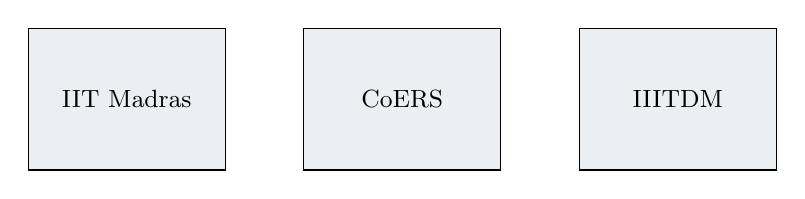
\begin{tikzpicture}
        \node[draw, rectangle, fill=lightgray, minimum width=2.5cm, minimum height=1.8cm] at (0,0) {\small IIT Madras};
        \node[draw, rectangle, fill=lightgray, minimum width=2.5cm, minimum height=1.8cm] at (3.5,0) {\small CoERS};
        \node[draw, rectangle, fill=lightgray, minimum width=2.5cm, minimum height=1.8cm] at (7,0) {\small IIITDM};
    \end{tikzpicture}
    
\end{center}
\end{frame}

\end{document}
